\documentclass[aspectratio=1610]{beamer}

\usetheme{unnslides}
\usefonttheme{professionalfonts}

\usepackage[T2A]{fontenc}
\usepackage[utf8]{inputenc}
\inputencoding{utf8}
\usepackage{listings}
\usepackage{graphicx}
\usepackage{caption}
\usepackage{cmbright}
\usepackage{fontspec}
\usepackage{unicode-math}
\usepackage{amsfonts}
\usepackage{subfig}
\usepackage{tikz}

\captionsetup[subfigure]{labelformat=empty}
\captionsetup[figure]{labelformat=empty}

\setmainfont{CMU Sans Serif}
\setromanfont{CMU Sans Serif}
\setsansfont{CMU Sans Serif}

\setlength{\tabcolsep}{1pt}

\usepackage{polyglossia}
\setmainlanguage{russian}
%\setbeamertemplate{itemize item}{\color{black}$\blacktriangleright$}

\DeclareMathOperator*{\argmax}{arg\,max}
\DeclareMathOperator*{\argmin}{arg\,min}
\DeclareMathOperator{\sign}{sign}
\DeclareMathOperator{\re}{Re}

\graphicspath{ {../pic/}{img/} }

%set pages numeration
\newcommand\numbered{\setbeamertemplate{footline}{%
  \vspace{-10em}
   \raisebox{5pt}{\makebox[\paperwidth]{%
     \hfill\makebox[10pt]{%
       \usebeamerfont{footline}\usebeamercolor[fg]{footline}
       \insertframenumber}}}}}
\newcommand\unnumbered{\setbeamertemplate{footline}{}}

\title{Parallel global optimization algorithm with uniform convergence
for solving a set of constrained global optimization problems}
\author{\underline{\textbf{V.V.~Sovrasov}} \and \textbf{K.A.~Barkalov}}
\institute{Nizhny Novgorod State University}
\date{}

\begin{document}
\numbered
{
\unnumbered
\begin{frame}[noframenumbering,plain]
\titlepage
\end{frame}
}

\begin{frame}
  \frametitle{Problem statement}
  \begin{columns}
    \begin{column}{0.5\textwidth}
      \begin{displaymath}
        \begin{array}{cr}\\
          \varphi(y^*)=\min\{\varphi(y):y\in D\}, \\
          D=\{y\in \mathbb{R}^N:a_i\leqslant y_i\leqslant{b_i}, \\ 1\leqslant{i}\leqslant{N},\:g_j(y)\leqslant 0, 1\leqslant j\leqslant m\}
        \end{array}
      \end{displaymath}
      \(\varphi(y),\:g_j(y)\) -- multi-extremal functions, satisfying the Lipschitz condition:
      \begin{displaymath}
        \begin{array}{cr}\\
          |f(y_1)-f(y_2)|\leqslant L\Vert y_1-y_2\Vert,\\y_1,y_2\in \mathbb{R}^N:a_i\leqslant y_i\leqslant{b_i},
        \end{array}
      \end{displaymath}
      where \(L>0\) is the Lipschitz constant and \(||\cdot||\) denotes the \(l_2\)-norm in \(\mathbb{R}^N\).
    \end{column}
    \begin{column}{0.5\textwidth}
      \centerline{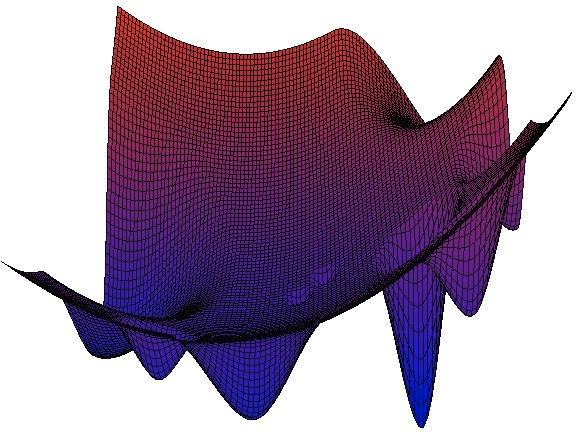
\includegraphics[width=0.9\textwidth]{img/gkls.png}}
    \end{column}
  \end{columns}
\end{frame}

\begin{frame}
  \frametitle{Problem statement}
  Let's consider a set of \(q\) global optimization problems with nonlinear constraints:
  \begin{displaymath}
    \min\left\{\varphi_1(y), y\in D_1 \right\}, \min\left\{\varphi_2(y), y\in D_2\right\},..., \min\left\{\varphi_q(y), y\in D_q\right\}.
  \end{displaymath}
  For an instance, such sets of problems can arise in the following cases:
  \begin{itemize}
    \item continuous global optimization problem with a discrete parameter which takes a narrow range of values;
    \item a set of problems, obtained after scalarization of a multi-objective problem.
  \end{itemize}
\textbf{Possible approaches}:
  \begin{itemize}
    \item solve each problem independently;
    \item develop an optimiaztion method, which solves all the problems "simultaneously", at each moment of time
    prioritizing one of the problems.
  \end{itemize}
\end{frame}

\begin{frame}
  \frametitle{Dimension reduction}
  \begin{center}
  Peano-type curve \(y(x)\) allows to reduce the dimension of the original problem:
  \begin{gather}
    D_e=\lbrace y\in \mathbb{R}^N:-2^{-1}\leqslant y_i\leqslant 2^{-1},1\leqslant i\leqslant N\rbrace=\{y(x):0\leqslant x\leqslant 1\} \nonumber \\
    \min\{\varphi(y): y\in D\}=\min\{\varphi(y(x)): x\in [0,1]\} \nonumber
  \end{gather}
  \(y(x)\) is non-smooth function which continuously maps the segment \([0,1]\) to the hypercube \(D_e\).
  \begin{figure}[ht]
    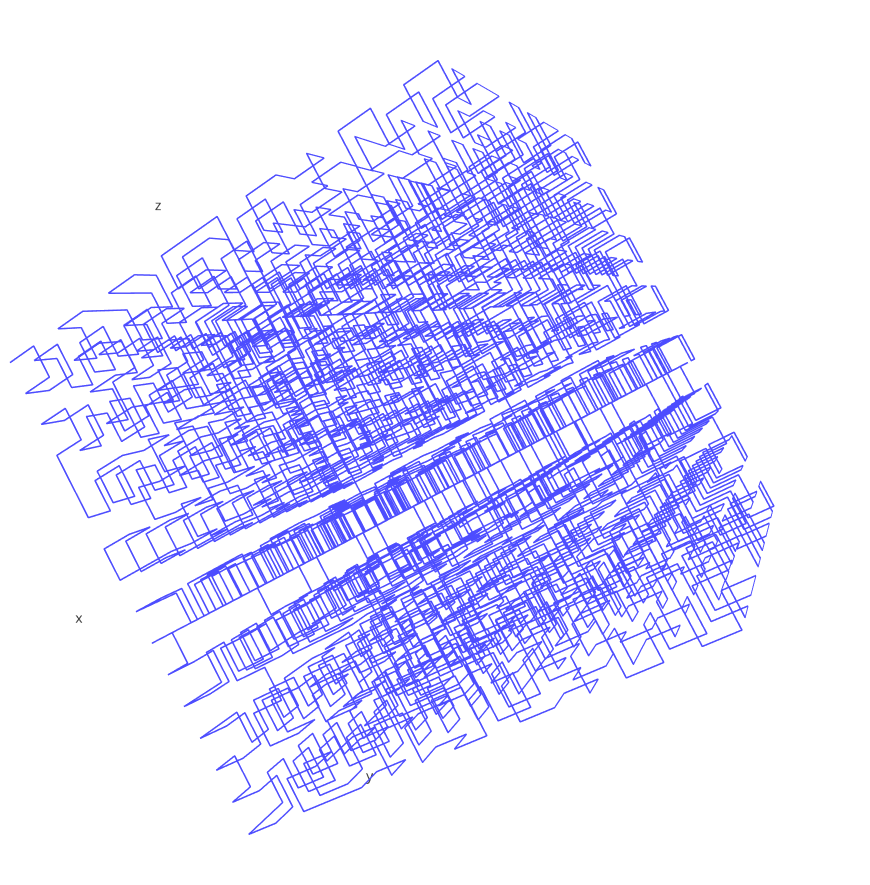
\includegraphics[width=.35\textwidth]{peano3d.png}
    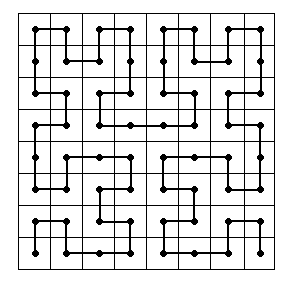
\includegraphics[width=.35\textwidth]{peano2d.png}
  \end{figure}
\end{center}
\end{frame}

\begin{frame}
  \frametitle{Univariate Algorithm of Global Search}
  Optimization method generates search sequence \(\{x_k:x_k\in[a,b]\}\) and consists of the following steps:
  \begin{enumerate}
    \setlength{\itemindent}{.1in}
    \item[Step 1.] Sort the search information (one-dimensional points) in increasing order.
    \item[Step 2.] For each interval \((x_{i-1}, x_i)\) compute quantity \(R(i)\), called characteristic.
    \item[Step 3.] Choose an interval with the greatest characteristic, \((x_{t-1}, x_{t})\), and
    make a trial (compute the constraints and objective) at the point \(x^{k+1}\), chosen according with decision rule \(d\):
    \begin{displaymath}
      x^{k+1}=d(t)\in (x_{t-1}, x_{t})
    \end{displaymath}
    \item[Step 4.] If \(x_{t}-x_{t-1}<\varepsilon\) stop the method.
  \end{enumerate}
  \textit{\footnotesize	{Detailed description: Strongin R.G., Sergeyev Ya.D.: Global optimization with non-convex constraints. Sequential and parallel algorithms (2000), Chapter 7}}
\end{frame}

\begin{frame}
  \frametitle{Algorithm for solving a set of problems}
  The method relies on the previously introduces AGS and consists of the following steps:
  \begin{itemize}
    \item Create \(q\) copies of AGS.
    \item Run \(q\) synchronously working copies of AGS, but instead of performing Step 3, stop all
    the methods and select an interval with the highest characteristic among intervals from all the methods.
    \item If the interval with the highest characteristic belongs to problem i \(i\), execute Step 3 in the \(i^{th}\) copy of AGS.
    Other copies skip Step 3.
    \item To implement parallel processing, method picks \(p\) intervals at the previous two steps
    and performs \(p\) trials simultaneously.
  \end{itemize}
  The described method relies to \textbf{comparability of characteristics in different problems}.
\end{frame}

\begin{frame}
  \frametitle{Index method of handling inequality constraints}
  Instead of the original problems with functional constraints the index scheme considers the following unconstrained problem:
  \begin{displaymath}
    \begin{array}{lr}
      \psi (x^{*})=\min_{x\in [0;1]}\psi (x), \\
      \psi (x)={\begin{cases}g_{\nu }(x)/H_{\nu }&\nu <M\\(g_{M}(x)-g_{M}^{*})/H_{M}&\nu =M\end{cases}},
    \end{array}
  \end{displaymath}
  where if \(\nu=m+1\;,g_\nu(x)=\varphi(x)\).

  Characteristics are defined as follows:
  \begin{displaymath}
    R(i)={\begin{cases}\Delta _{i}+{\frac {(z_{i}-z_{i-1})^{2}}{(r_{\nu }\mu _{\nu })^{2}\Delta _{i}}}-2{\frac {z_{i}+z_{i-1}-2z_{\nu }^{*}}{r_{\nu }\mu _{\nu }}}&\nu =\nu (x_{i})=\nu (x_{i-1})\\2\Delta _{i}-4{\frac {z_{i-1}-z_{\nu }^{*}}{r_{\nu }\mu _{\nu }}}&\nu =\nu (x_{i-1})>\nu (x_{i})\\2\Delta _{i}-4{\frac {z_{i}-z_{\nu }^{*}}{r_{\nu }\mu _{\nu }}}&\nu =\nu (x_{i})>\nu (x_{i-1})\end{cases}}
  \end{displaymath}
  where \(z_i=\psi(x_i)\).
\end{frame}

\begin{frame}
  \frametitle{Index method of handling inequality constraints}
\end{frame}

\begin{frame}
  \frametitle{Пример решения многокритериальной задачи}
  Рассматриваемая задача:
  \begin{displaymath}
    \begin{array}{l}
        Minimize \left \{
        \begin{array}{l}
          f_1(y) = 4 y_1^2 + 4 y_2^2 \\
          f_2(y) = (y_1-5)^2 + (y_2-5)^2 \\
        \end{array}
        \right .
        y_1\in [-1;2],y_2\in [-2;1]
        \\s.t.
        \\
        \left \{
        \begin{array}{l}
          g_1(y) = (y_1 - 5)^2 + y_2^2 - 25 \leqslant 0 \\
          g_2(y) = -(y_1 - 8)^2 - (y_2 + 3)^2 + 7.7 \leqslant 0\\
        \end{array}
        \right .
    \end{array}
  \end{displaymath}
  После использования свёртки Гермейера для скаляризации задача примет вид:
  \begin{displaymath}
    \varphi(y^*(\lambda_1,\lambda_2))=\min_{y\in D}\max\{\lambda_1 f_1(y), \lambda_2 f_2(y)\};\lambda_1,\lambda_2\in[0,1],\: \lambda_1+\lambda_2=1
\end{displaymath}
Для численного построения множества Парето выберем
100 наборов коэффициентов \((\lambda_1,\lambda_2)\) таких, что
\(\lambda_1^i=i h,\: \lambda_2^i=1-\lambda_1^i,\: h=10^{-2},i=\overline{1, 100}\).
\end{frame}

\begin{frame}
  \frametitle{Пример решения многокритериальной задачи}
  \vspace*{-1.0cm}
  \begin{displaymath}
    \begin{array}{cr}\\
      SP(S)=\sqrt{\frac{1}{|S|-1} \sum_{i=1}^{|S|} (\overline{d}-d_i)^2},\:\overline{d}=mean\{d_i\}, \\
      d_i=\min_{s_i,s_j\in S:s_i\ne s_j}||F(s_i)-F(s_j)||_1,\: F=(f_1,f_2)
    \end{array}
  \end{displaymath}

  \begin{figure}[ht]
      \centering
      \vspace*{-0.5cm}
      \subfloat[Раздельное решение задач, \(SP_{single}=0.984\)]{
      \label{fig:mco_pareto_1} {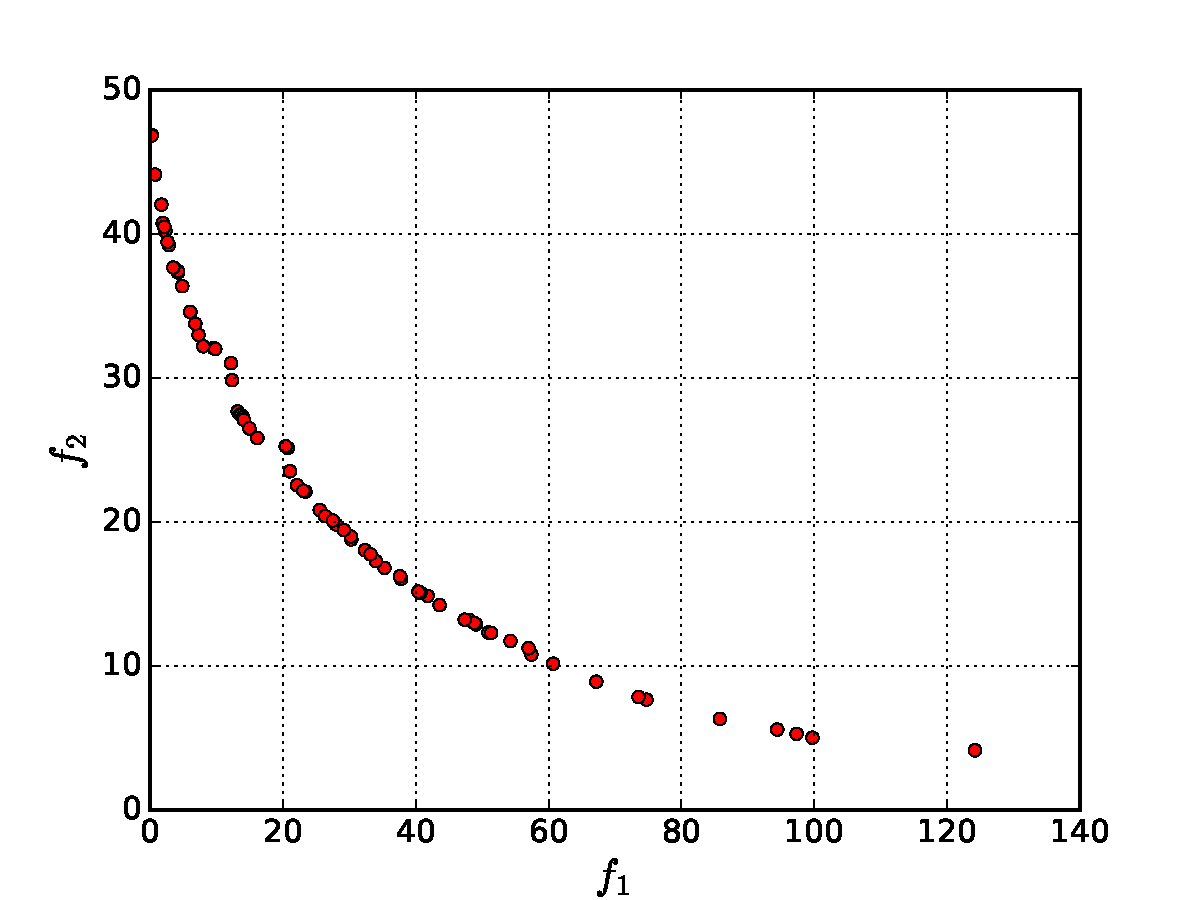
\includegraphics[width=.5\textwidth]{single_mco.pdf}}}
      \subfloat[Решение множества задач, \(SP_{multi}=0.749\)]{
      \label{fig:mco_pareto_2} {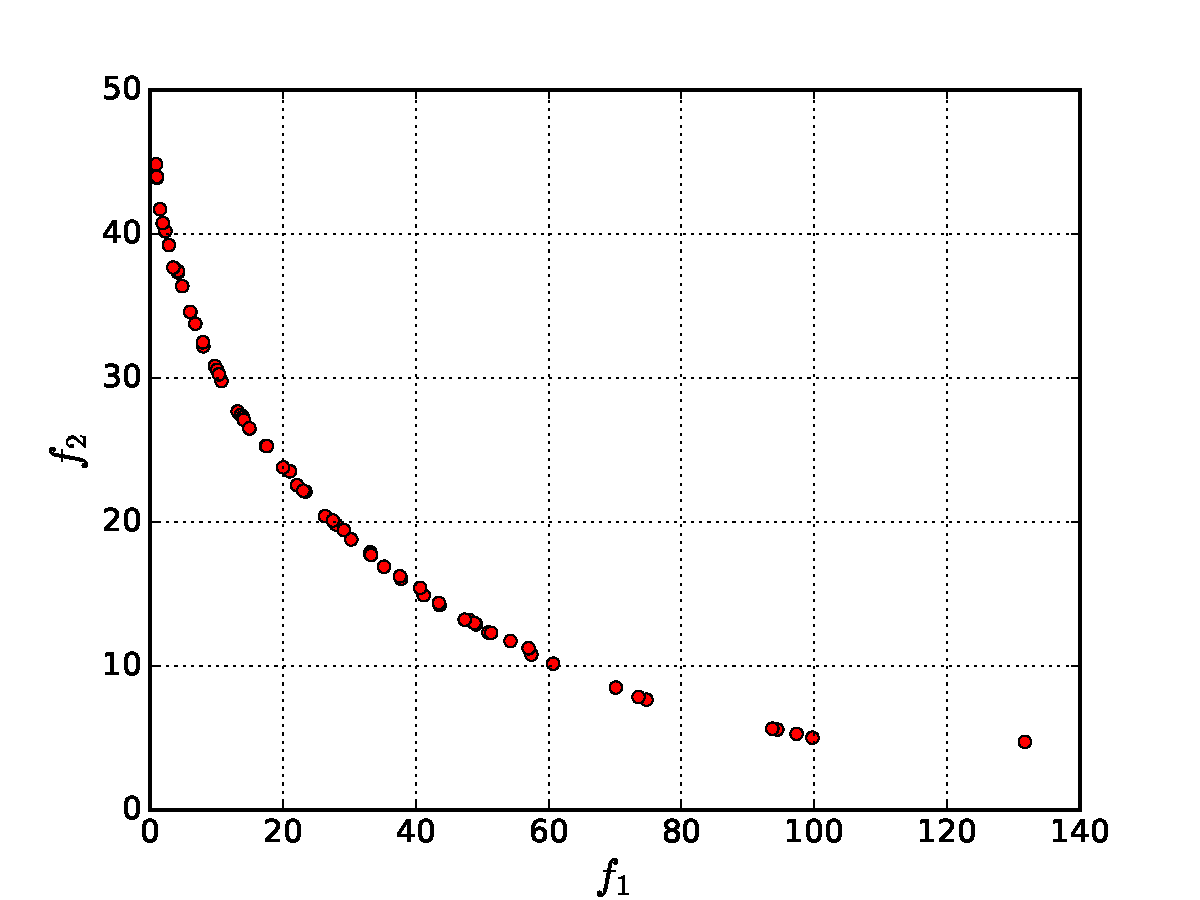
\includegraphics[width=.5\textwidth]{multi_mco.pdf}}}
      \caption{Численные оценки множества Парето, полученные после 2500 испытаний}
      \label{fig:mco_pareto}
  \end{figure}
\end{frame}

\begin{frame}
  \frametitle{Тестовые многомерные задачи с ограничениями}
  \begin{columns}
    \begin{column}{0.5\textwidth}
      Тестовые наборы были получены с помощью системы GCGen, позволяющей
      сторить многомерные задачи с ограничениями из заданных функций, и нескольких
      известных генераторов тестовых задач (GKLS, \(F_{GR}\)).
      Характеристики каждого из сгенерированных наборов задач:
      \begin{itemize}
        \item \(q\)=100;
        \item Размерность 2 или 3;
        \item Базовые функции только GKLS или \(F_{GR}\), или их комбинация;
        \item Количество ограничений: 2.
      \end{itemize}
    \end{column}
    \begin{column}{0.5\textwidth}
      \centerline{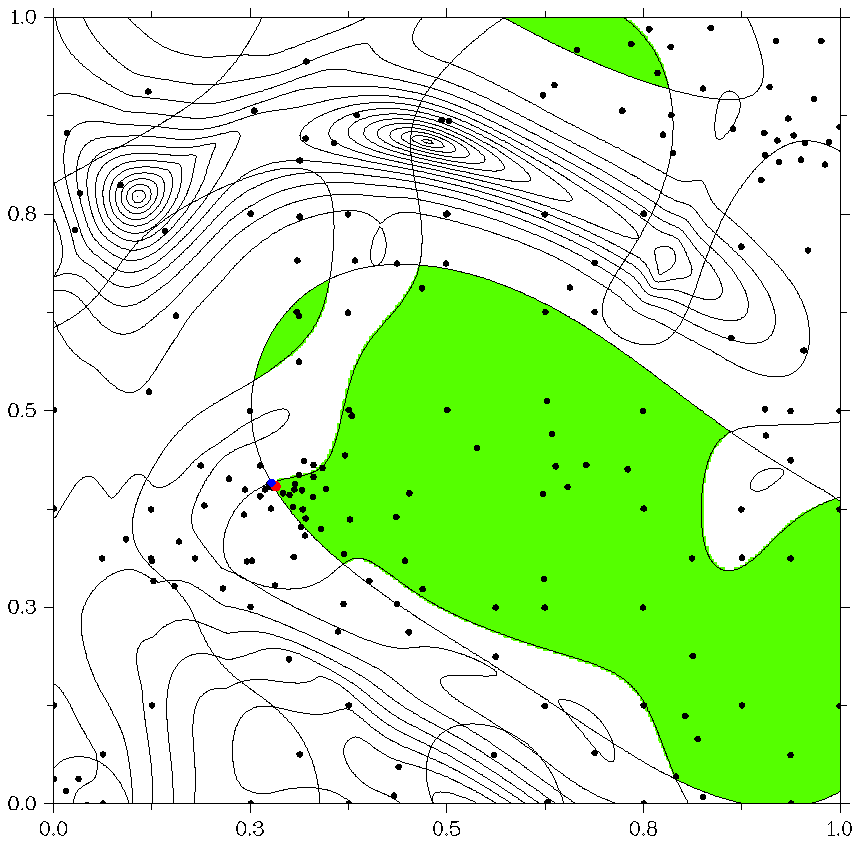
\includegraphics[width=0.9\textwidth]{4.png}}
    \end{column}
  \end{columns}
  \footnotesize{Система GCGen доступна по ссылке \textit{https://github.com/UNN-ITMM-Software/GCGen}}
\end{frame}

\begin{frame}
  \frametitle{Программное и техническое обеспечение}
  \begin{center}
    Реализация параллельного метода была выполнена на языке C++ с использованием технологии OpenMP
    для распареллеливания процесса проведения испытаний на общей памяти.

    Все вычислительные
    эксперименты проведены на машине со следующей конфигурацией: Intel Core i7-7800X (6 cores) CPU, 64GB RAM, Unubtu 16.04 ОS, GCC 5.5 compiler.
  \end{center}
\end{frame}

\begin{frame}
  \frametitle{Результаты экспериментов на наборах синтетических задач}
  \begin{figure}[ht]
    \vspace*{-0.5cm}
      \centering
      \subfloat[\(D_{max}\)]{
      \label{fig:max_dev} {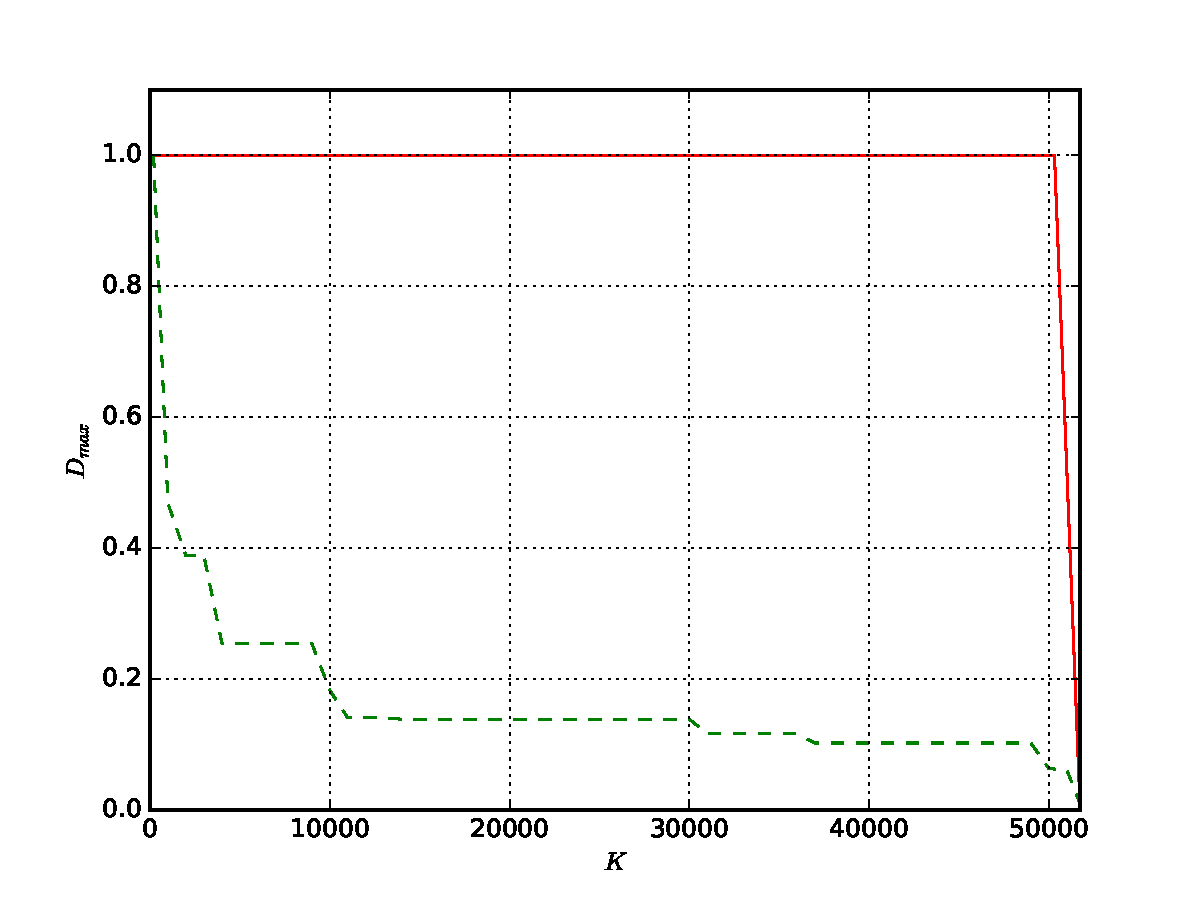
\includegraphics[width=.5\textwidth]{mixed_2d_max.pdf}}}
      \subfloat[\(D_{avg}\)]{
      \label{fig:avg_dev} {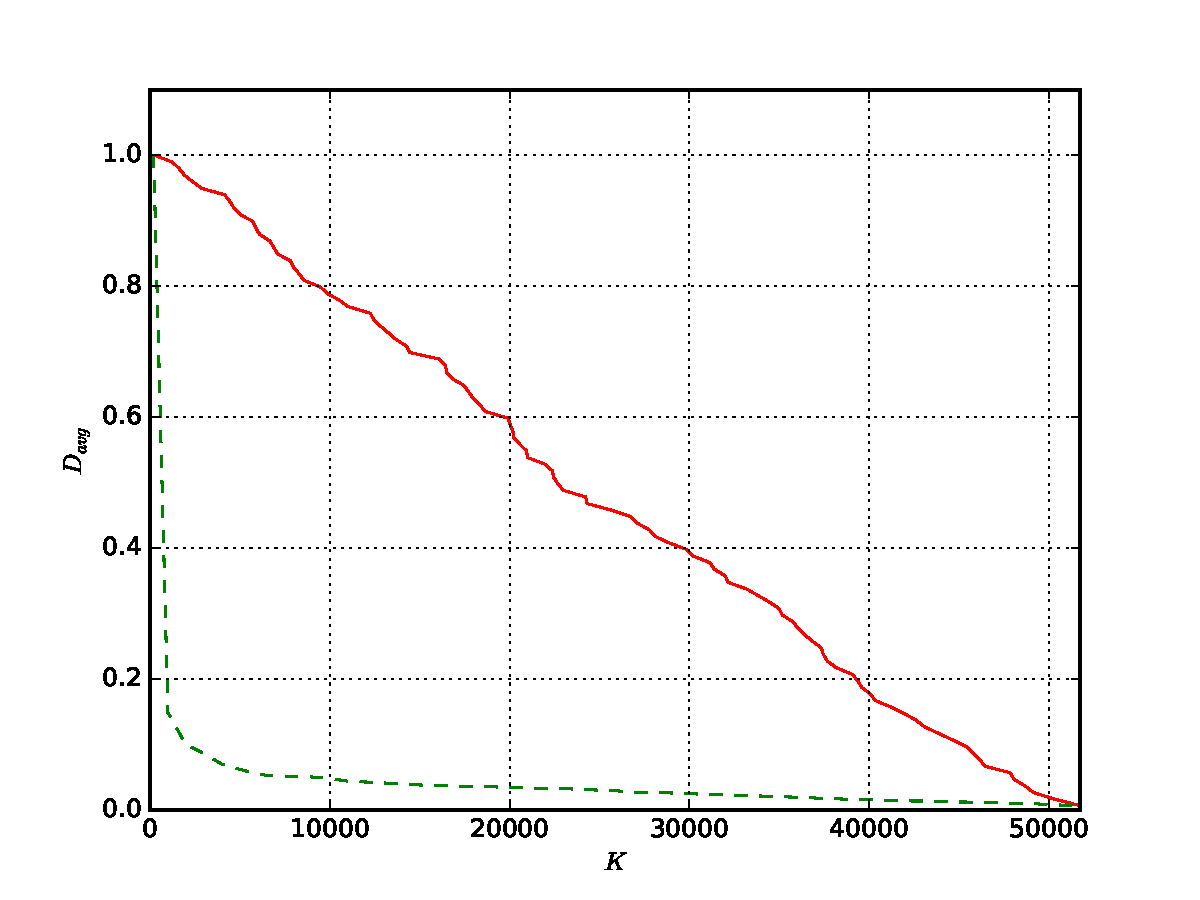
\includegraphics[width=.5\textwidth]{mixed_2d_avg.pdf}}}
      \caption{Динамика величин средней по задачам и максимальной точности в процессе решения множества двухмерных задач,
      порождённых двумя разными генераторами GKLS и \(F_{GR}\)}
      \label{fig:devs_mixed}
  \end{figure}
\end{frame}

\begin{frame}
  \frametitle{Результаты экспериментов на наборах синтетических задач}
  \begin{table}
    \centering
    \begin{tabular}{c|c|c|c|c|c}
      %\cline{1-8}\noalign{\smallskip}
      Класс задач & \textit{p} & Количество итераций & Время, с & \(S_i\) & \(S_t\)   \\
      %s\noalign{\smallskip} \cline{4-5} \cline{7-8}  \noalign{\smallskip}
      \hline
      GKLS \& \(F_{GR}\)-based \
        & 1 & 51434 & 90.20 & -    & - \\
        & 2 & 25698 & 56.96 & 2.00 & 1.58 \\
        & 4 & 13015 & 36.67 & 3.95 & 2.46 \\
        & 6 & 8332  & 26.85 & 6.17 & 3.36 \\
      \hline
      GKLS-based 2d \
        & 1 & 59066 & 97.53 & -    & - \\
        & 2 & 29060 & 60.56 & 2.04 & 1.61 \\
        & 4 & 14266 & 38.92 & 4.14 & 2.51 \\
        & 6 & 9436  & 29.53 & 6.26 & 3.30 \\
      \hline
      GKLS-based 3d \
        & 1 & 782544 & 1117.55 & -    & - \\
        & 2 & 397565 & 752.92  & 1.97 & 1.48 \\
        & 4 & 208073 & 526.67  & 3.76 & 2.12 \\
        & 6 & 142089 & 445.45  & 5.50 & 2.51 \\
      \hline
    \end{tabular}
  \end{table}
\end{frame}

\begin{frame}
  \frametitle{Заключение}
  В ходе работы были достигнуты следующие результаты:
    \begin{itemize}
      \item реализована поддержка нелинейных ограничений в алгоритме, решающeм
      множество задач глобальной оптимизации;
      \item проведены численные эксперименты, демонстрирующие преимущество рассматриваемого подхода в скорости сходимости на всём множестве задач в среднем над решением задач по отдельности;
      \item показана эффективность совместного решения множества задач на примере решения многокритериальной задачи с нелинейными ограничениями.
    \end{itemize}

    В ходе дальнейшей работы планируется:
    \begin{itemize}
      \item улучшить текущую реализацию алгоритма, сократив расходы на содержание поисковой информации для множества задач и тем самым улучшив
      показатели параллельного ускорения по времени;
      \item реализовать версию рассматриваемого алгоритма, работающего на распределенной памяти.
    \end{itemize}
\end{frame}

{
\unnumbered
\begin{frame}{{}}
  \frametitle{Q\&A}
  \begin{center}
    \Large{Контакты:}
\vspace{0.5cm}

    sovrasov.vlad@gmail.com

    https://github.com/sovrasov
  \end{center}
\end{frame}
}
\end{document}
